\chapter{Authentication and Access Control}

\section*{Introduction}
This chapter presents the first release of the PMS platform. Its purpose is to make the application
usable and secure before any business functionality is built on top of it. It opens with the
preparation phase, six weeks of study that preceded the first line of production code, and then
gathers two sprints: Sprint~1 establishes the technical foundation and the authentication chain,
Sprint~2 delivers the dynamic authorization model together with the management of users and
resources.

At the end of this release the platform authenticates its users, applies a configurable
authorization policy, and holds the reference data, that is users, resources and cost rates, which
the operational modules of the next release consume.

% =====================================================================
\section{Release 1 backlog}
The first release realises the seven user stories of the product backlog
(Table~\ref{tab:backlog}) that concern access to the platform. Because the author is the sole
developer, each story is expanded into the technical work it required.

\begin{longtable}{|m{1.5cm}|m{6.8cm}|m{5.2cm}|m{1.4cm}|}
\hline
\textbf{Story} & \textbf{Need} & \textbf{Technical work} & \textbf{Sprint} \\
\hline
\endhead
\endfoot
\endlastfoot
\hline
US-01 & Sign in with an e-mail and a password & Authentication service, BCrypt verification, JWT
issuance signed with HMAC-SHA512, refresh cookie, token rotation & 1 \\
\hline
US-02 & Be forced to change an imposed password on first login & \texttt{first\_login} flag,
dedicated filter restricting the token to the password-change endpoint & 1 \\
\hline
US-03 & Revoke a user's sessions immediately & Token version persisted per user, embedded in each
token and compared on every request & 1 \\
\hline
US-04 & Assign permissions to roles without redeploying & \texttt{roles}, \texttt{permissions} and
\texttt{role\_permissions} tables, permissions carried in the token and converted into Spring
Security authorities & 2 \\
\hline
US-05 & See only the menu entries the account is entitled to & Context endpoint returning the held
permissions, navigation built from that response & 2 \\
\hline
US-06 & Create, modify and deactivate user accounts & User module, creation with a temporary
password, activation state, role assignment & 2 \\
\hline
US-07 & Record resources and their yearly cost rate & Resource entity separate from the account,
loaded cost rate stored per resource and per year & 2 \\
\hline
\caption{Backlog of release 1}
\label{tab:backlog-r1}
\end{longtable}

% =====================================================================
\section{Preparation phase}
The release opens with six weeks that produced no production code. They ran from 5~January to
13~February and are listed as such in the schedule of Chapter~2
(Table~\ref{tab:schedule}). Their purpose was to arrive at the first sprint already knowing what
had to be built, on which architecture, and what it should look like.

\subsection{What the phase produced}
Four deliverables came out of it, each of which is presented in full elsewhere in this report and
only summarised here.

\begin{itemize}
  \item \textbf{The reading of the existing instrument.} The project review workbook was opened
        sheet by sheet, its formulas traced, and its business rules written down. This is the
        analysis of Chapter~1, and it is the reason the platform reproduces the company's financial
        model rather than an approximation of it.
  \item \textbf{The requirements and the product backlog.} The rules extracted from the workbook
        were turned into actors, functional and non-functional requirements, and twenty-five user
        stories distributed across four releases. This is Chapter~2.
  \item \textbf{The architecture and the technical stack.} The modular monolith, the dynamic
        authorization model, the hybrid indicator engine and the relational schema were decided
        before any of them was written. This is Chapter~3.
  \item \textbf{The interface models.} Screen models were produced for the main workflows, so that
        the sprints could be spent implementing an agreed interface rather than inventing one under
        time pressure. These models are the subject of the rest of this section.
\end{itemize}

\subsection{Interface models}
The models were produced with \textbf{Google Stitch}, a generative interface design tool: each
screen is described in natural language and the tool returns a working layout that can then be
refined. It was chosen for a reason specific to this project, which had a single developer and no
designer. Producing a credible screen in minutes rather than days made it affordable to explore
several arrangements of the same information, and to discard the ones that did not work before any
of them cost a sprint.

Two things should be said plainly about these models. They carry a provisional product name,
\emph{ProjectControl}, and amounts in euros, because they were exploratory sketches rather than
specifications; the delivered platform is named PMS and reports in Tunisian dinars. And they are
models of \emph{layout and information hierarchy} only: no model describes a permission, a
computation or a state transition, all of which come from the analysis rather than from the design
tool.

\subsubsection{Sign-in}
The entry point of the platform was the first screen modelled, because it is the only one every
user sees and the only one seen before any authorization applies.

\begin{figure}[H]
  \centering
  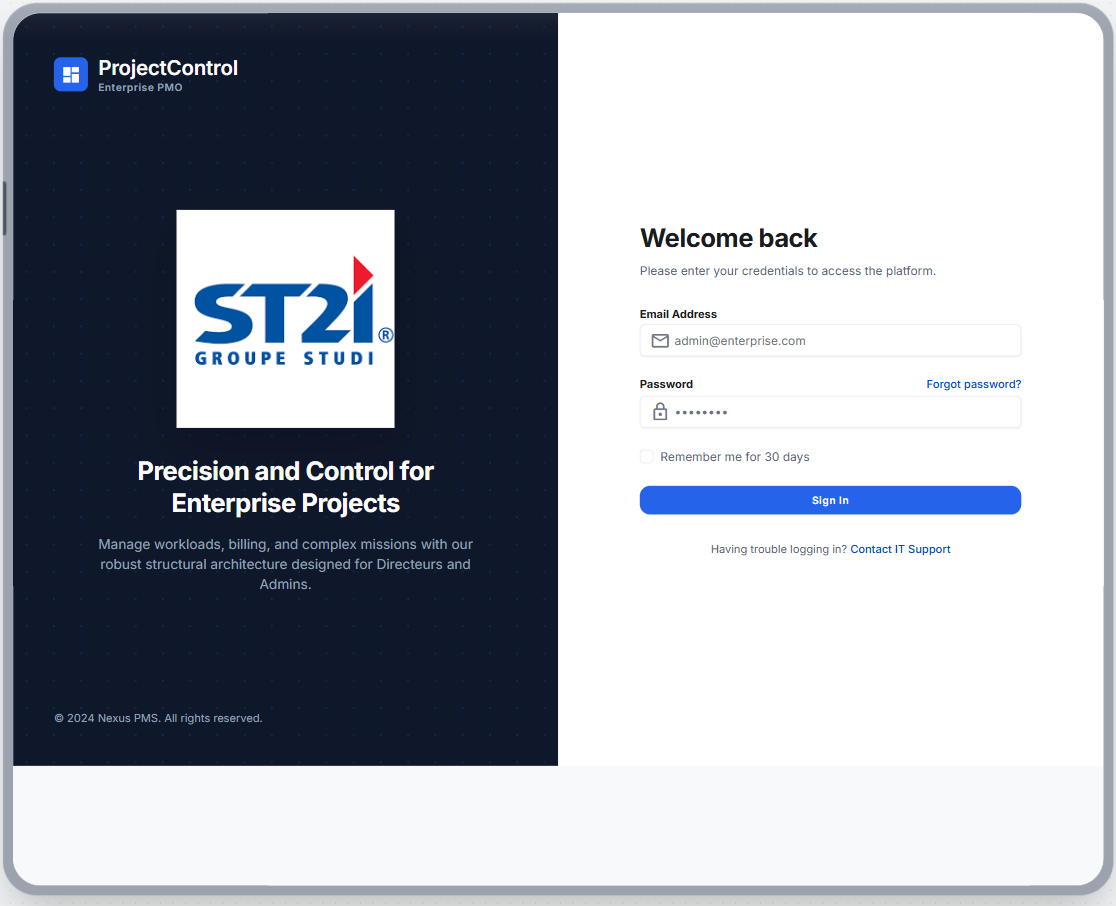
\includegraphics[width=0.88\columnwidth]{img/mk_login.png}
  \caption{Interface model --- sign-in screen}
  \label{fig:mk-login}
\end{figure}

\subsubsection{Steering screens}
The director reads the portfolio; the project manager reads one project in depth. The models
separated those two readings from the start, which is what later became the portfolio dashboard and
the per-project indicator board of Sprint~8.

\begin{figure}[H]
  \centering
  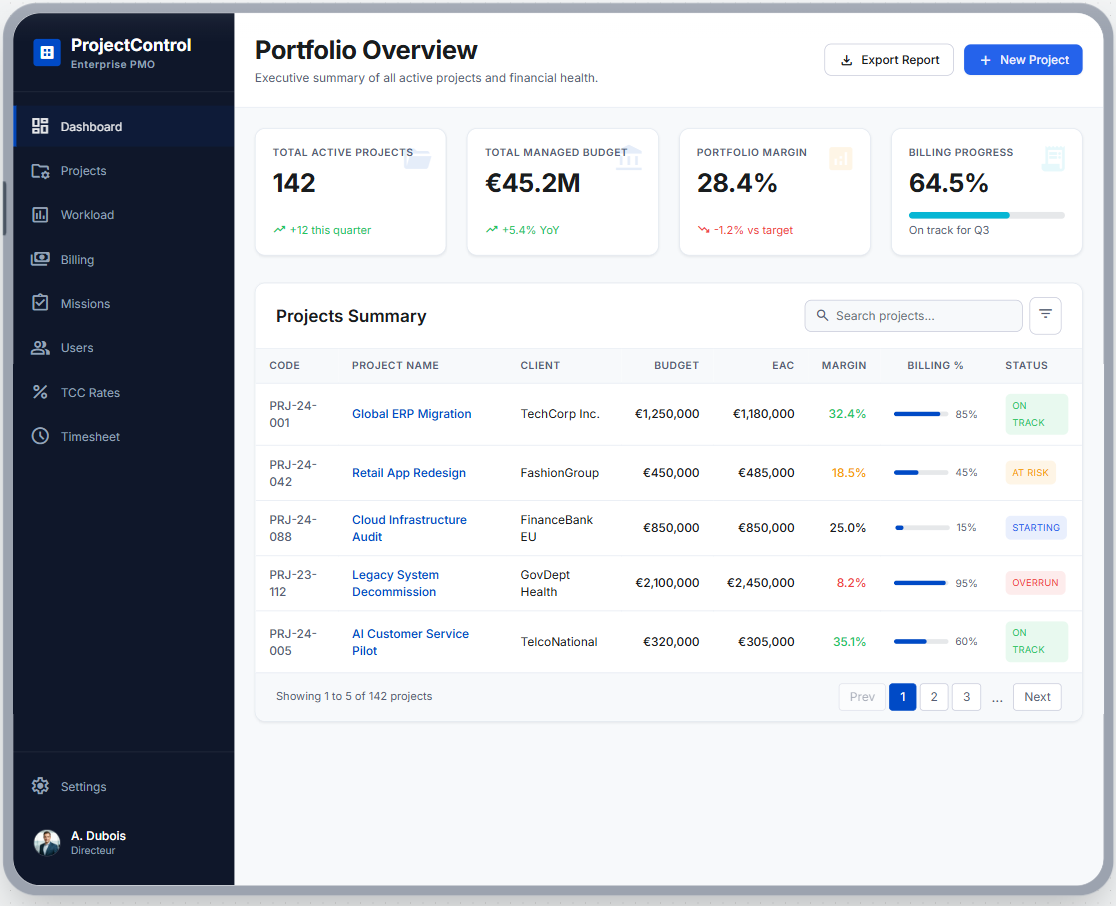
\includegraphics[width=0.88\columnwidth]{img/mk_portfolio.png}
  \caption{Interface model --- portfolio overview for the director}
  \label{fig:mk-portfolio}
\end{figure}

\begin{figure}[H]
  \centering
  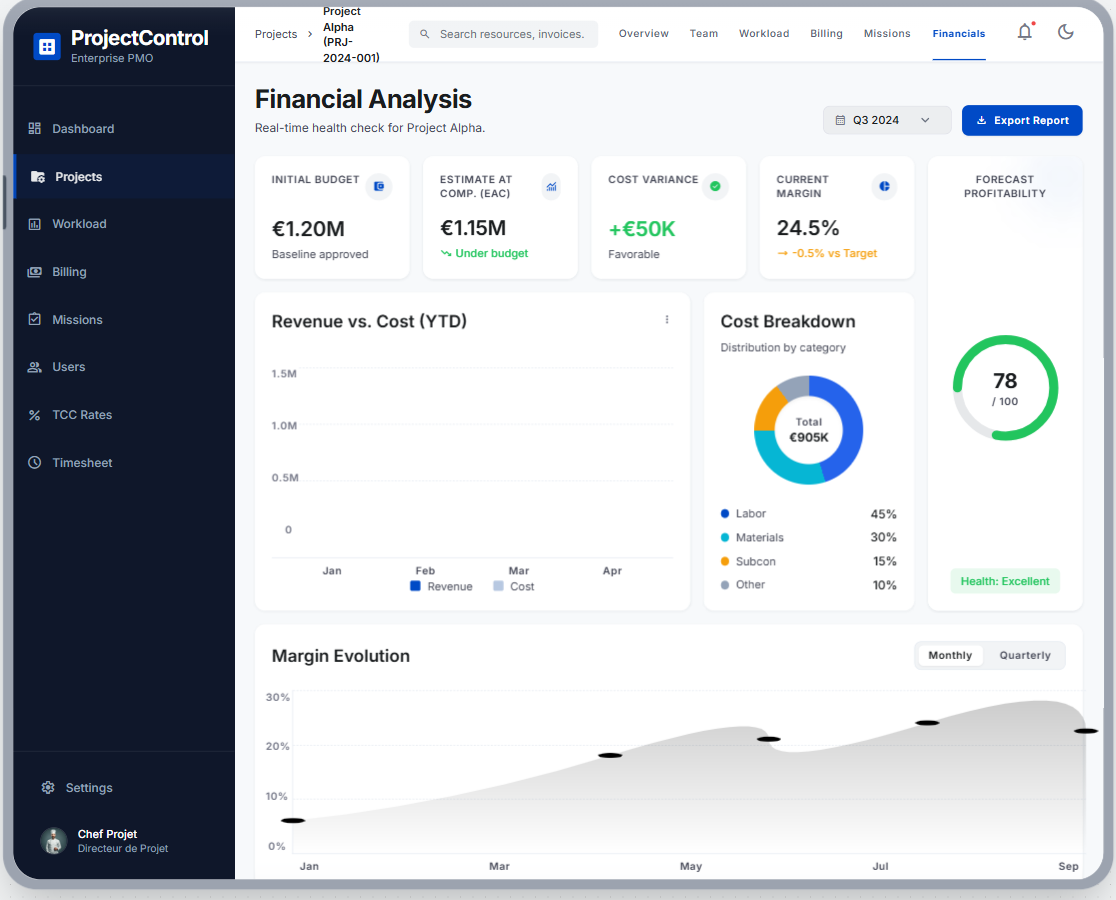
\includegraphics[width=0.88\columnwidth]{img/mk_financial.png}
  \caption{Interface model --- financial analysis of a single project}
  \label{fig:mk-financial}
\end{figure}

\subsubsection{Operational screens}
The workload matrix and the billing timeline are the two screens that carry the most business
logic, and both were modelled before being built.

\begin{figure}[H]
  \centering
  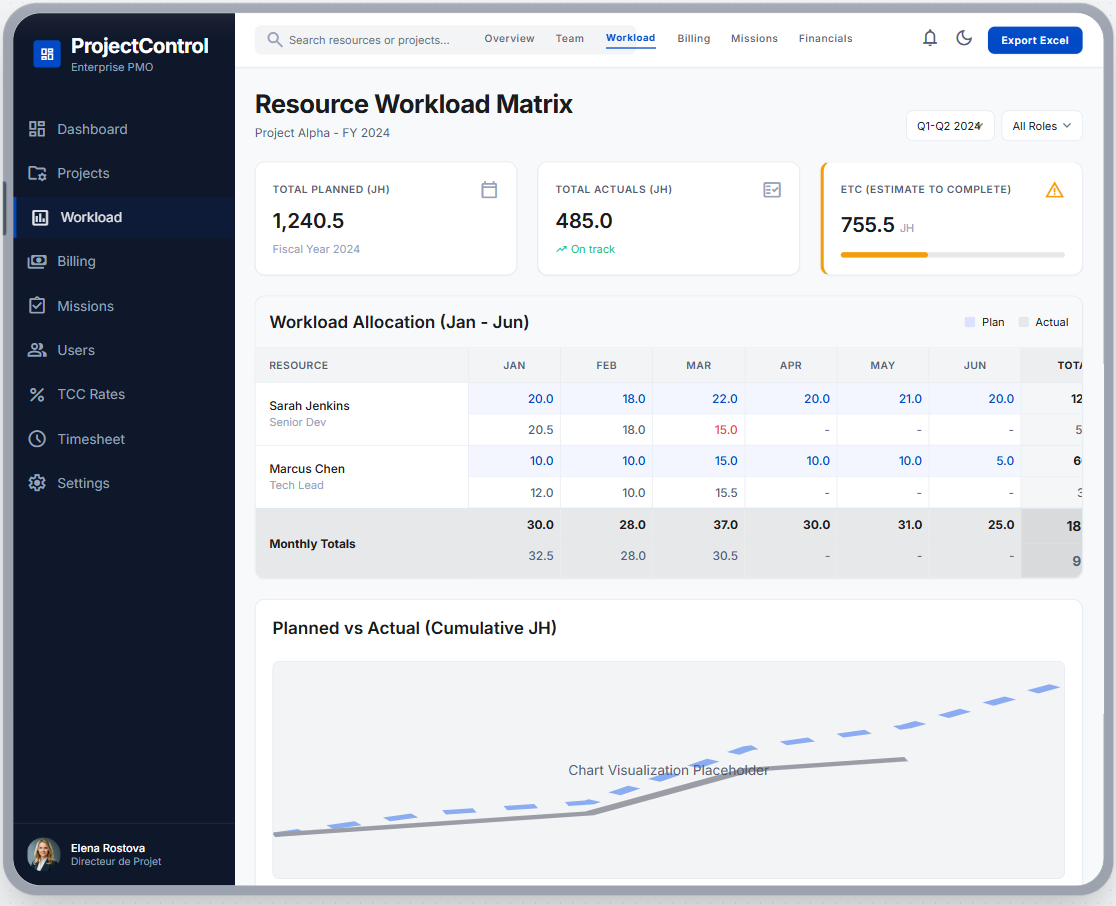
\includegraphics[width=0.88\columnwidth]{img/mk_workload.png}
  \caption{Interface model --- resource workload matrix, planned against actual}
  \label{fig:mk-workload}
\end{figure}

\begin{figure}[H]
  \centering
  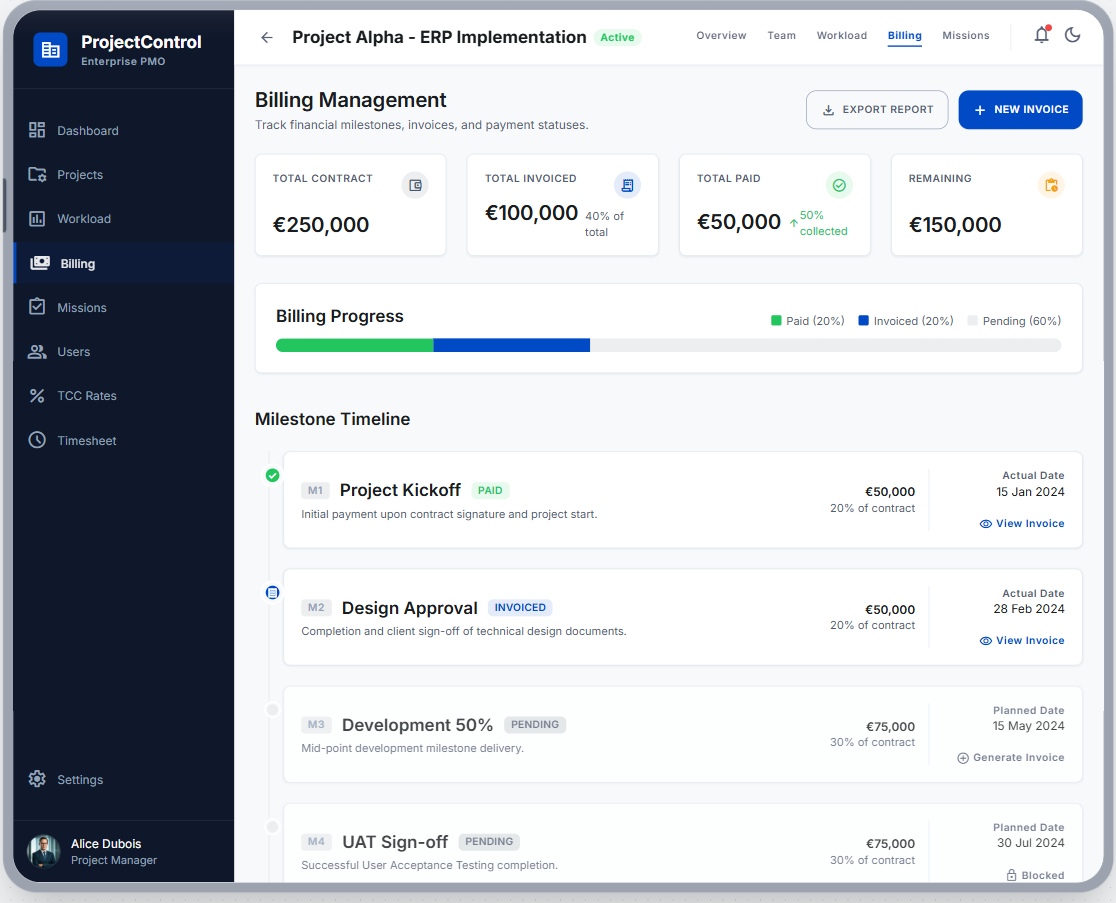
\includegraphics[width=0.88\columnwidth]{img/mk_billing.png}
  \caption{Interface model --- billing milestones and their progress}
  \label{fig:mk-billing}
\end{figure}

\subsubsection{Screens of the restricted roles}
Modelling the developer and administrator views early was what made the consequence of the
authorization model visible before it was implemented: a role that holds few permissions does not
get a reduced version of the same screen, it gets a different and much shorter menu.

\begin{figure}[H]
  \centering
  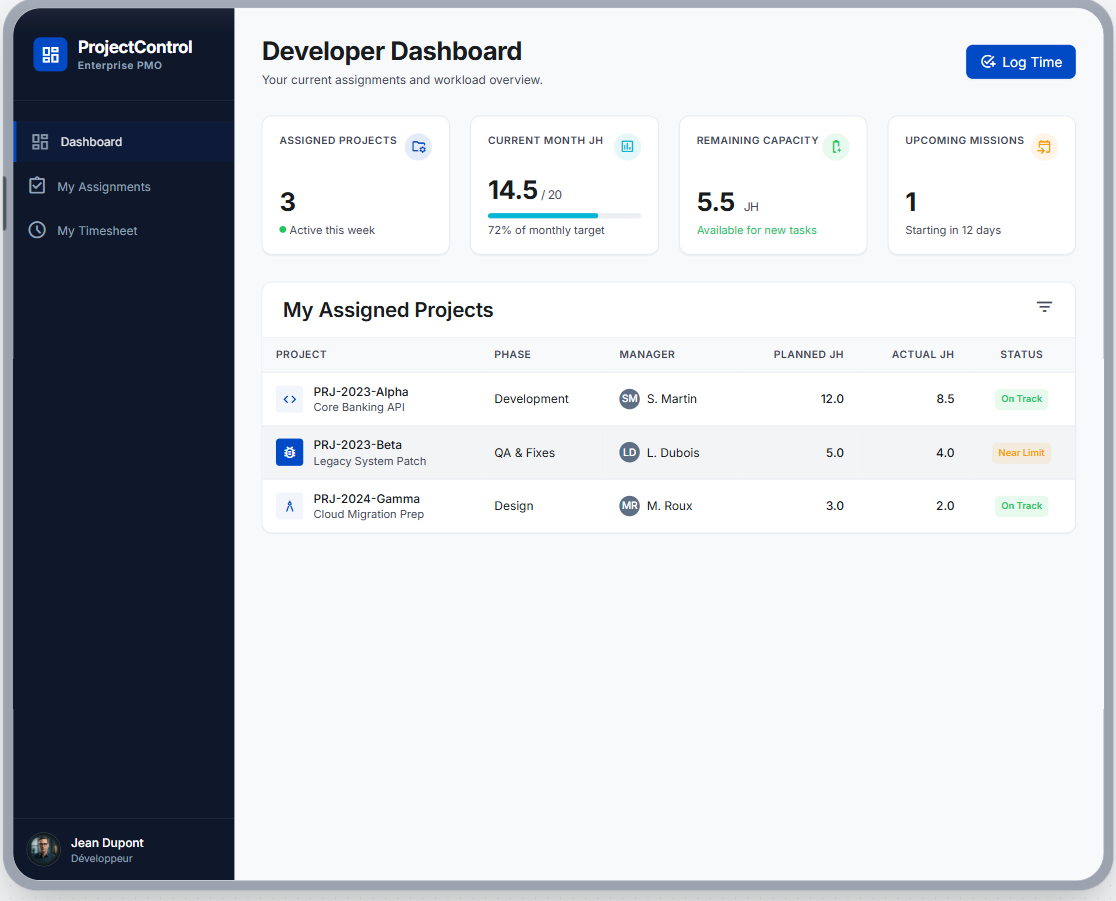
\includegraphics[width=0.88\columnwidth]{img/mk_developer.png}
  \caption{Interface model --- developer workspace, reduced to assignments and time entry}
  \label{fig:mk-developer}
\end{figure}

\begin{figure}[H]
  \centering
  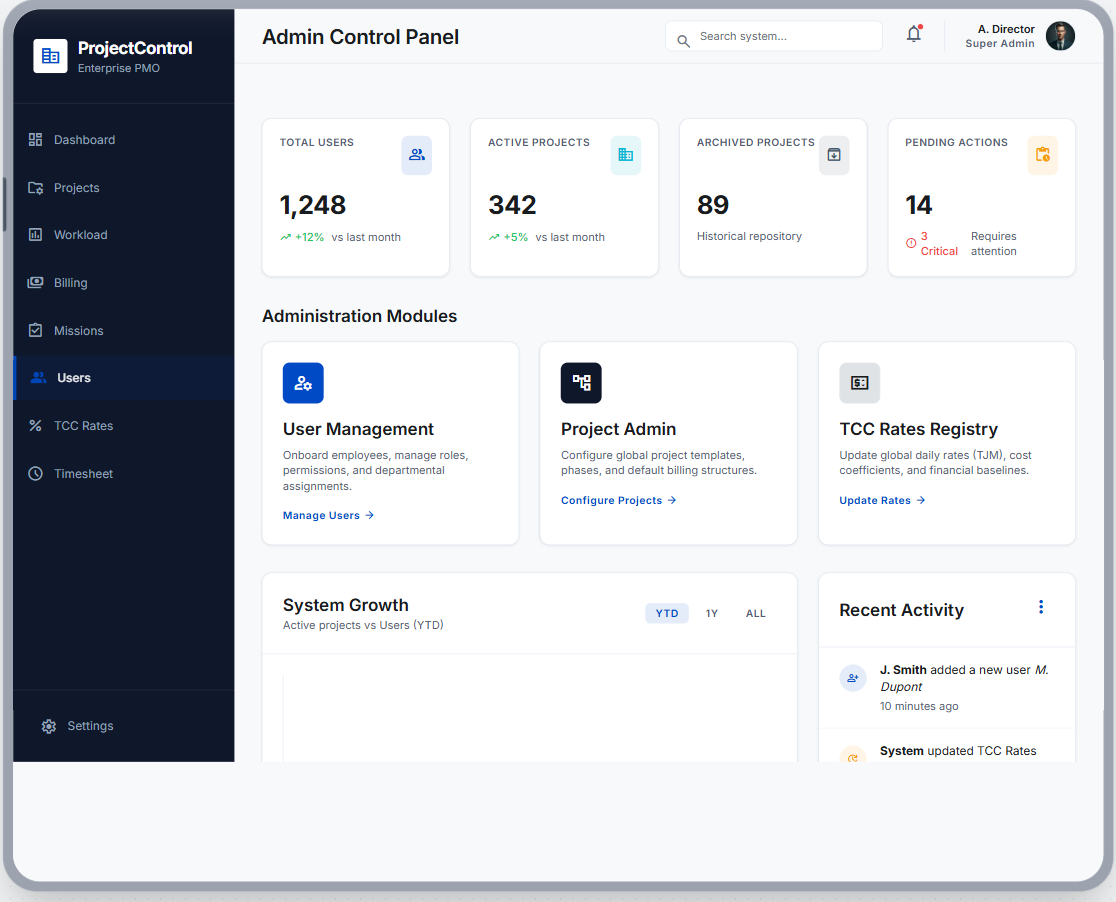
\includegraphics[width=0.88\columnwidth]{img/mk_admin.png}
  \caption{Interface model --- administration panel}
  \label{fig:mk-admin}
\end{figure}

\subsection{From the models to the delivered interface}
Table~\ref{tab:model-traceability} follows each model through to the screen that was actually
delivered, and records where the two diverge. The divergences are the useful part: they are the
places where implementation taught something the model could not.

\begin{longtable}{|m{3.5cm}|m{3.4cm}|m{7.0cm}|}
\hline
\textbf{Model} & \textbf{Delivered screen} & \textbf{What changed, and why} \\
\hline
\endhead
\endfoot
\endlastfoot
\hline
Sign-in (Fig.~\ref{fig:mk-login}) & Fig.~\ref{fig:ui-login} & Kept almost unchanged. The forced
password change on first login was added, because it comes from a security requirement the model
did not express. \\
\hline
Portfolio overview (Fig.~\ref{fig:mk-portfolio}) & Fig.~\ref{fig:ui-portfolio} & The summary tiles
survived. The flat project table became a ranking by margin with a portfolio health bar, because
a director scanning eighty projects needs the worst ones first, not the newest. \\
\hline
Financial analysis (Fig.~\ref{fig:mk-financial}) & Fig.~\ref{fig:ui-kpi} & The indicator set was
replaced by the one the workbook actually defines: EAC, ETC, accrued income and drift in man-days,
rather than the generic cost breakdown the model proposed. \\
\hline
Workload matrix (Fig.~\ref{fig:mk-workload}) & Fig.~\ref{fig:ui-workload} & Confirmed. The
planned-against-actual matrix by resource and by month is the arrangement the workbook already
used, and the model made it visible early enough to build it once. \\
\hline
Billing (Fig.~\ref{fig:mk-billing}) & Fig.~\ref{fig:ui-billing} & The vertical timeline became a
table. A milestone is compared with its neighbours far more often than it is read on its own, and a
table compares better than a timeline. \\
\hline
Developer workspace (Fig.~\ref{fig:mk-developer}) & Fig.~\ref{fig:ui-dev-dashboard} & Confirmed in
shape, and made a consequence of the permission model rather than a separate screen: the menu is
built from the permissions the account holds. \\
\hline
Administration (Fig.~\ref{fig:mk-admin}) & Figs.~\ref{fig:ui-users} and~\ref{fig:ui-perm-catalogue}
& Split in two. The single panel of the model hid the distinction the platform rests on, between
managing accounts and editing the authorization policy. \\
\hline
\caption{From the interface models to the delivered screens}
\label{tab:model-traceability}
\end{longtable}

The phase closed with the development environment in place: the repository, the database, the
migration tool and the build, so that the first sprint began with a running, empty application
rather than with its installation.

% =====================================================================
\section{Sprint 1 --- Authentication and technical foundation}

\subsection{Sprint 1 use case diagram}
The sprint covers the three use cases that every user must traverse before reaching a business
screen: authenticating, changing an imposed password, and terminating a session. Every other use
case of the platform includes authentication, which is why this sprint precedes all the others.

\begin{figure}[H]
  \centering
  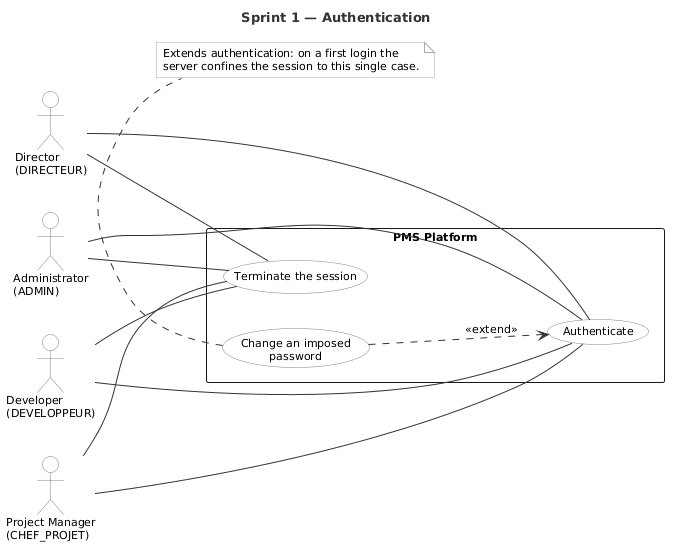
\includegraphics[width=0.75\columnwidth]{img/uc_sprint1.png}
  \caption{Use case diagram of sprint 1}
  \label{fig:uc-s1}
\end{figure}

\subsection{Sprint 1 analysis and design}

\subsubsection{Sequence of the ``Authenticate'' use case}
The nominal scenario involves the browser, the authentication controller, the authentication
service, the token service and the user repository. It shows where the password is verified, where
the two tokens are produced, and why only one of them is written to a cookie.

\begin{figure}[H]
  \centering
  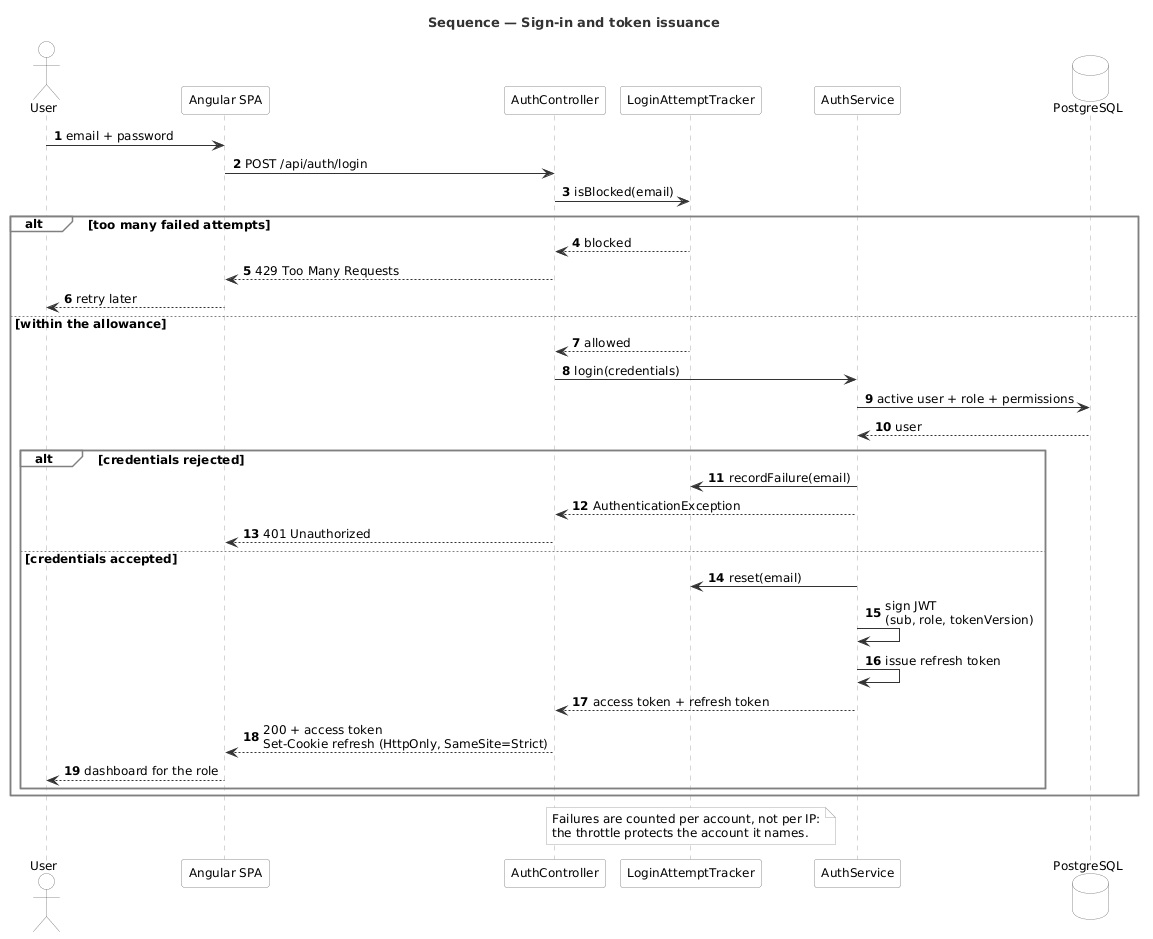
\includegraphics[width=0.95\columnwidth]{img/seq_s1_login.png}
  \caption{Sequence diagram of the ``Authenticate'' use case}
  \label{fig:seq-s1-login}
\end{figure}

\subsubsection{Sequence of the ``Change the password on first login'' use case}
An account created by the administrator carries a temporary password. The scenario shows how the
token issued at the first connection is restricted, how any business call is refused while the flag
remains set, and how a full token is issued once the password has been changed.

\begin{figure}[H]
  \centering
  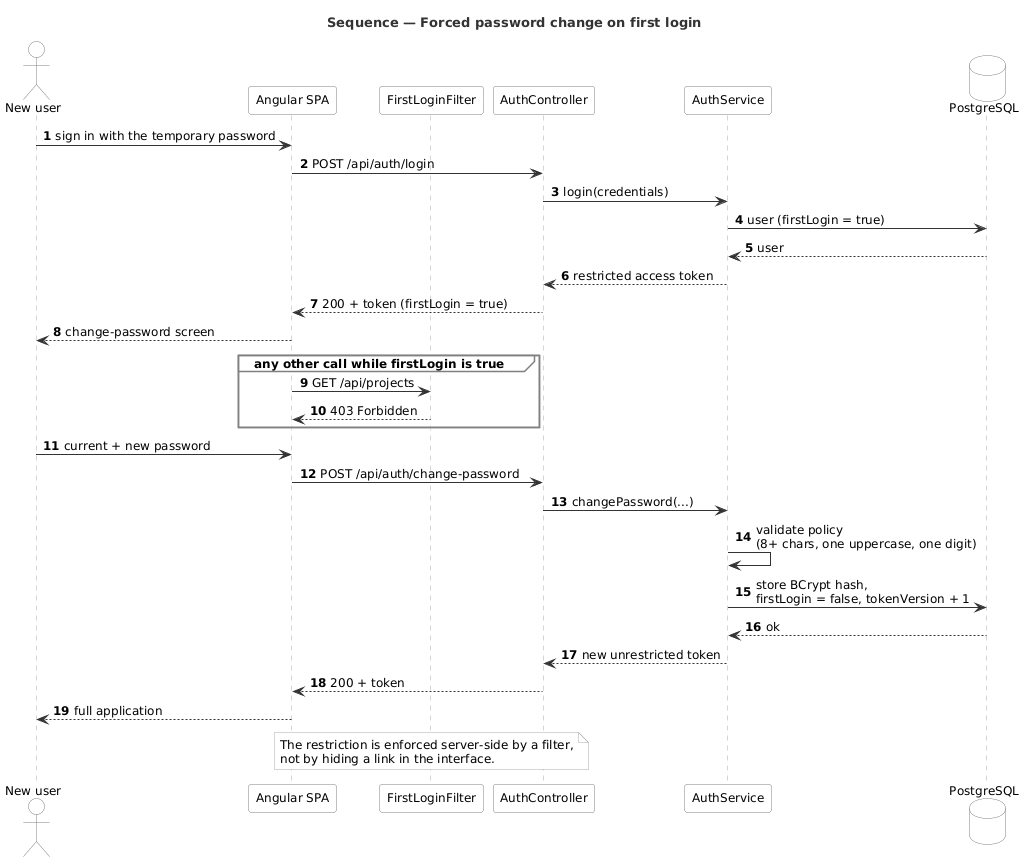
\includegraphics[width=0.95\columnwidth]{img/seq_s1_first_login.png}
  \caption{Sequence diagram of the ``Change the password on first login'' use case}
  \label{fig:seq-s1-first}
\end{figure}

\subsubsection{Sequence of the ``Revoke a session'' use case}
Revocation is the scenario that justifies the design of the token. It shows the increment of the
version, the invalidation of the cache entry, and the rejection of a request presenting a token
issued before the increment.

\begin{figure}[H]
  \centering
  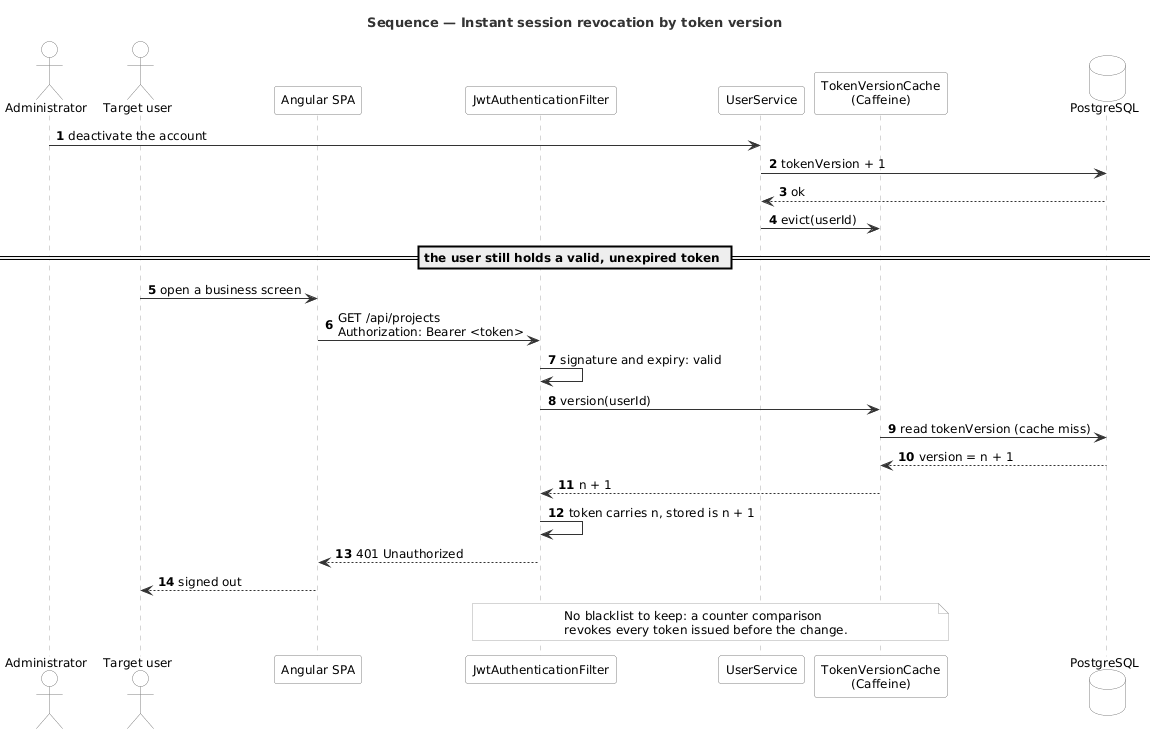
\includegraphics[width=0.95\columnwidth]{img/seq_s1_revoke.png}
  \caption{Sequence diagram of the ``Revoke a session'' use case}
  \label{fig:seq-s1-revoke}
\end{figure}

\subsubsection{Design decisions}
Three decisions taken in this sprint constrain the whole platform and are therefore justified here
rather than in the realisation.

\textbf{A modular monolith rather than services.} The code is organised into independent functional
packages, each with its own Controller $\rightarrow$ Service $\rightarrow$ Repository $\rightarrow$
Domain layering. A single deployable artefact keeps transactions local and avoids distributed
consistency, which matters because the financial computations of release~3 read from several
modules within one transaction. The package boundaries preserve the option of extraction later.

\textbf{Two tokens rather than one.} A short-lived access token held in memory is paired with a
refresh token confined to an \texttt{HttpOnly} cookie. A single long-lived token stored in the
browser would be readable by any injected script; splitting them means the credential able to mint
new sessions is never reachable from JavaScript. The refresh token is additionally rotated on every
use, so a stolen cookie stops working as soon as the legitimate holder refreshes.

\textbf{Revocation by version rather than by blacklist.} A JWT is self-contained and cannot be
withdrawn once issued. A server-side blacklist would reintroduce the shared state that the stateless
design avoids. Storing a single integer per user and embedding it in each token achieves the same
result: incrementing it invalidates every session of that identity at once, at the cost of one
integer comparison per request.

\subsection{Sprint 1 realization}

\subsubsection{Modular monolith structure}
The modules are \texttt{auth}, \texttt{user}, \texttt{project}, \texttt{team}, \texttt{workload},
\texttt{agile}, \texttt{kpi}, \texttt{billing}, \texttt{mission}, \texttt{governance} and
\texttt{shared}. Each subsequent sprint adds its module without modifying the previous ones.

\subsubsection{Base entity and automatic auditing}
All business entities inherit from \texttt{BaseEntity}, which centralises the auto-generated primary
key, the \texttt{createdAt} and \texttt{updatedAt} timestamps managed by \texttt{@PrePersist} and
\texttt{@PreUpdate}, and the \texttt{deleted} marker implementing logical deletion. No data is ever
physically erased, and every repository implicitly filters on \texttt{deleted = false}. This
satisfies the auditability requirement (NFR-008).

\subsubsection{Schema management through Flyway}
The database structure is managed exclusively by Flyway. Hibernate never emits implicit DDL: the
property \texttt{spring.jpa.\allowbreak hibernate.\allowbreak ddl-auto} is set to \texttt{validate},
so a divergence between the entities and the schema stops the application at startup rather than
corrupting data at runtime. The versioned migrations are idempotent and constitute the living
documentation of the schema.

\subsubsection{Token issuance and rotation}
On \texttt{POST /api/auth/login} the authentication service verifies the e-mail, compares the
supplied password with the BCrypt hash, checks that the account is active, then issues a short-lived
JWT access token signed with \texttt{HMAC-SHA512} carrying the e-mail, the token version and the
list of permission codes, together with a refresh token placed in the protected cookie.

\texttt{POST /api/auth/refresh} exchanges a valid cookie for a new access token and a new refresh
cookie; the previous one is rejected from that moment on.

\subsubsection{Immediate revocation by token version}
Revocation rests on a \texttt{token\_version} field persisted in the \texttt{users} table and
embedded in every issued token. On each request the \texttt{JwtAuthenticationFilter} compares the
version carried by the token with the value read from an in-memory cache; if they differ the request
is rejected with \texttt{401 Unauthorized}. Incrementing the field therefore closes every active
session of that identity instantly, which is what happens on logout and on password change, the
latter also terminating sessions opened on other devices.

\subsubsection{Protection against repeated failures}
\texttt{LoginAttemptTracker} counts consecutive failures per identity and temporarily refuses
further attempts, answering \texttt{429 Too Many Requests}. Password guessing is therefore bounded
without locking a legitimate account permanently.

\subsubsection{Forced password change on first login}
When an account is created the administrator sets a temporary password and \texttt{first\_login} is
set to \texttt{true}. The token issued at the first connection carries a restricted right enforced
by \texttt{FirstLoginFilter}: only \texttt{POST /api/\allowbreak auth/\allowbreak change-password}
is authorised. Once the password is changed, \texttt{first\_login} becomes \texttt{false} and an
unrestricted token is issued.

\begin{figure}[H]
  \centering
  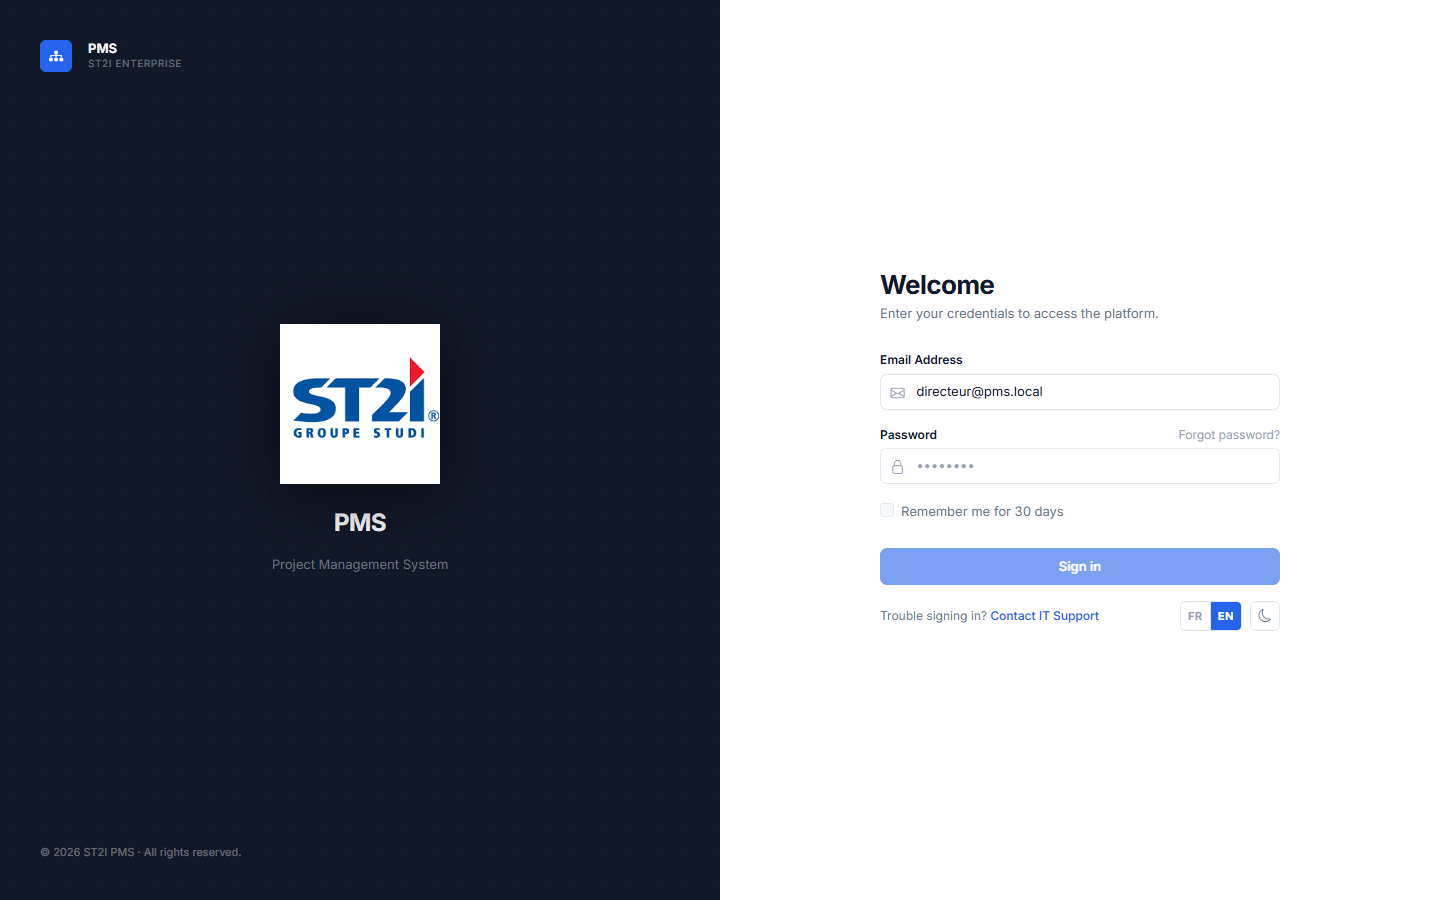
\includegraphics[width=0.8\columnwidth]{img/ui_login.png}
  \caption{Login interface}
  \label{fig:ui-login}
\end{figure}

\emph{\small Note on the screenshots. Every screen reproduced in this chapter and the following
ones was captured against a demonstration dataset generated for the purpose. The project codes,
client names, staff names and amounts they show are fictitious and correspond to no real engagement
of the host organization. No production data appears in this document.}

\begin{figure}[H]
  \centering
  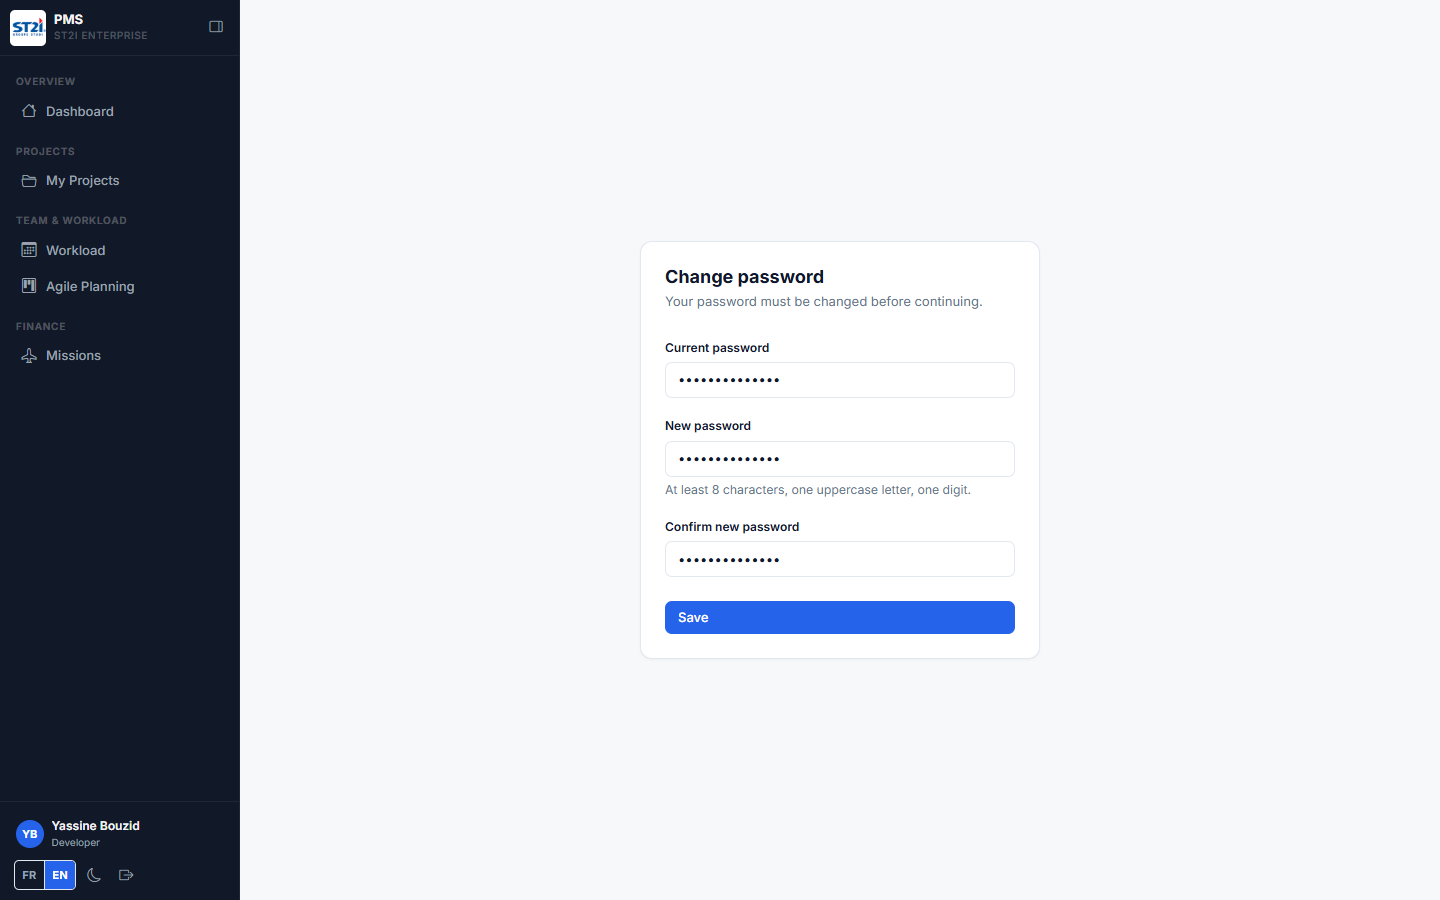
\includegraphics[width=0.8\columnwidth]{img/ui_change_password.png}
  \caption{Forced password change interface}
  \label{fig:ui-change-password}
\end{figure}

% =====================================================================
\section{Sprint 2 --- Dynamic access control, users and resources}

\subsection{Sprint 2 use case diagram}
The sprint covers the administration use cases: assigning permissions to a role, managing user
accounts, and recording resources with their yearly cost rate. All of them are reserved to the
administrator, and all of them include the authentication delivered by sprint~1.

\begin{figure}[H]
  \centering
  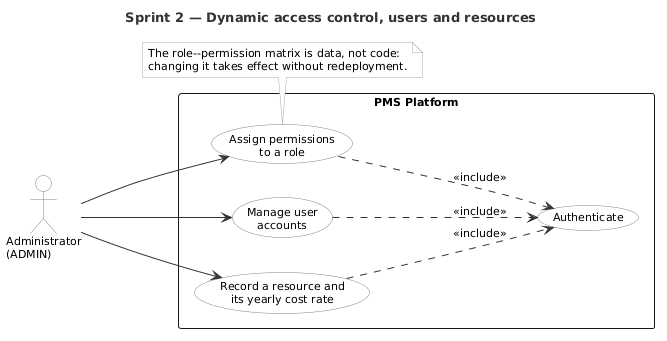
\includegraphics[width=0.75\columnwidth]{img/uc_sprint2.png}
  \caption{Use case diagram of sprint 2}
  \label{fig:uc-s2}
\end{figure}

\subsection{Sprint 2 analysis and design}

\subsubsection{Model of the authorization policy}
The authorization model is the structuring design of the platform and deserves its own class
diagram. A role aggregates permissions, a permission belongs to a functional module, and a user
holds one active role. Nothing in this model is compiled into the application: the association
between a role and its permissions is a table, so the policy is data.

\begin{figure}[H]
  \centering
  
\includegraphics[width=0.85\columnwidth]{img/class_rbac.png}
  \caption{Class diagram of the authorization model}
  \label{fig:class-rbac}
\end{figure}

\subsubsection{Sequence of the ``Grant a permission to a role'' use case}
This scenario is the proof that the policy is configurable. It shows the administrator adding a
permission to a role, the association being persisted, and the affected users obtaining the new
right on their next token without any redeployment.

\begin{figure}[H]
  \centering
  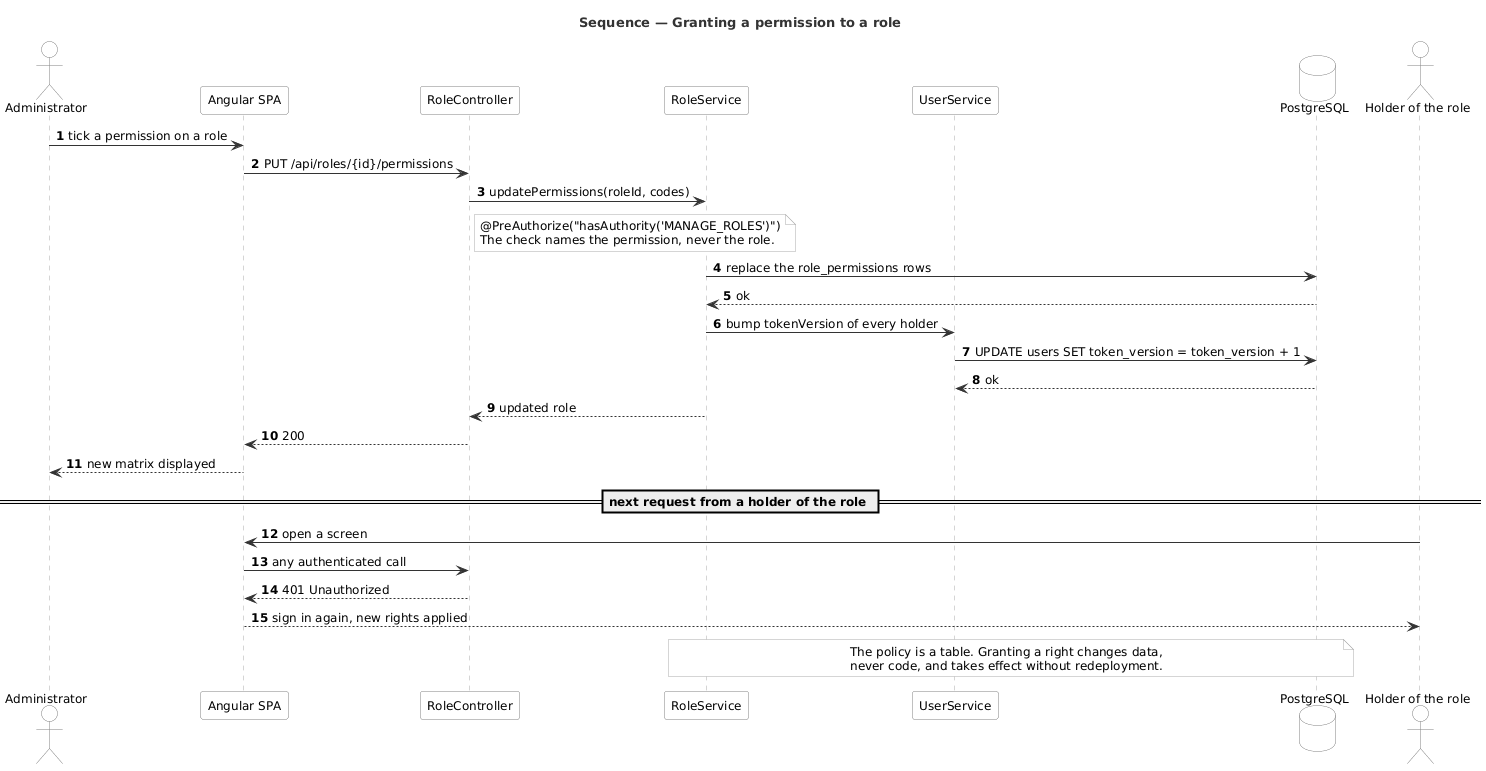
\includegraphics[width=0.95\columnwidth]{img/seq_s2_grant_permission.png}
  \caption{Sequence diagram of the ``Grant a permission to a role'' use case}
  \label{fig:seq-s2-grant}
\end{figure}

\subsubsection{Design decisions}
\textbf{Permissions rather than roles in the code.} No role name is ever tested in the application.
Only permission codes are, through annotations of the form
\texttt{@PreAuthorize("hasAuthority('CREATE\_PROJECT')")}. Testing a role would hard-code the policy
into the source and make every change a release; testing a permission leaves the policy in the
database.

\textbf{A resource is not an account.} A resource represents a cost-bearing capacity and may exist
without a platform account, since the workbook records people who never connect to any system.
Merging the two notions would have made it impossible to cost a contributor who has no login.

\textbf{A cost rate per year, not per resource.} The loaded cost rate is recorded per resource
\emph{and per year}, so that the cost of a man-day uses the rate of the year in which the effort was
booked. This requirement comes directly from the workbook, where the 2024 and 2025 rates of the same
person differ.

\subsection{Sprint 2 realization}

\subsubsection{Permission, role and user model}
The \texttt{role\_permissions} table associates a set of permissions with a role. A user holds a
single active role, but that role can be reconfigured at any time by the administrator without
redeployment. A dedicated migration initialises the four default roles, Administrator, Director,
Project Manager and Developer, with eighteen permission codes spread over seven functional modules.

\subsubsection{Propagation to Spring Security}
The \texttt{JwtAuthenticationFilter} reads the permission codes from the token and converts them
into \texttt{SimpleGrantedAuthority} objects, after which every REST entry point is protected by its
\texttt{@PreAuthorize} annotation.

\subsubsection{Dynamic menu}
The context endpoint returns, for the authenticated user, the list of their permissions together
with their profile information. The Angular frontend builds the navigation menu from that response:
an item is displayed only if the user holds the required permission code. The interface therefore
reflects the authorization policy automatically, with no duplicated rule on the client side.

Figures~\ref{fig:ui-perm-catalogue} to~\ref{fig:ui-dev-dashboard} show the effect on the same
build of the application, signed in as three different roles. The permission catalogue states the
policy; the two dashboards show what it produces.

\begin{figure}[H]
  \centering
  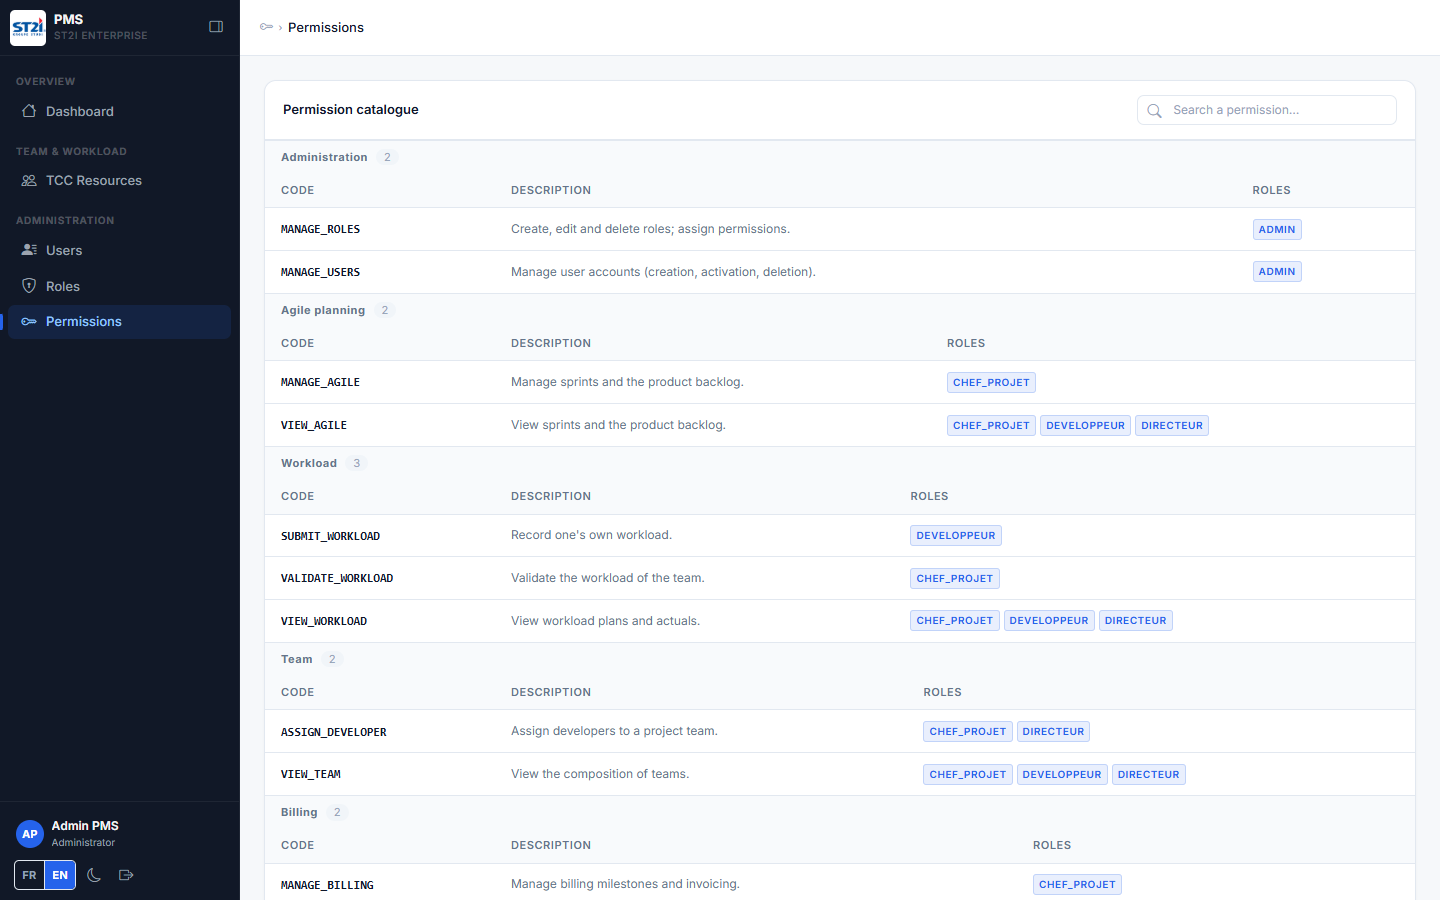
\includegraphics[width=0.92\columnwidth]{img/ui_permissions.png}
  \caption{Permission catalogue: the policy as the administrator reads it, grouped by functional
           module, with the roles that hold each code}
  \label{fig:ui-perm-catalogue}
\end{figure}

\begin{figure}[H]
  \centering
  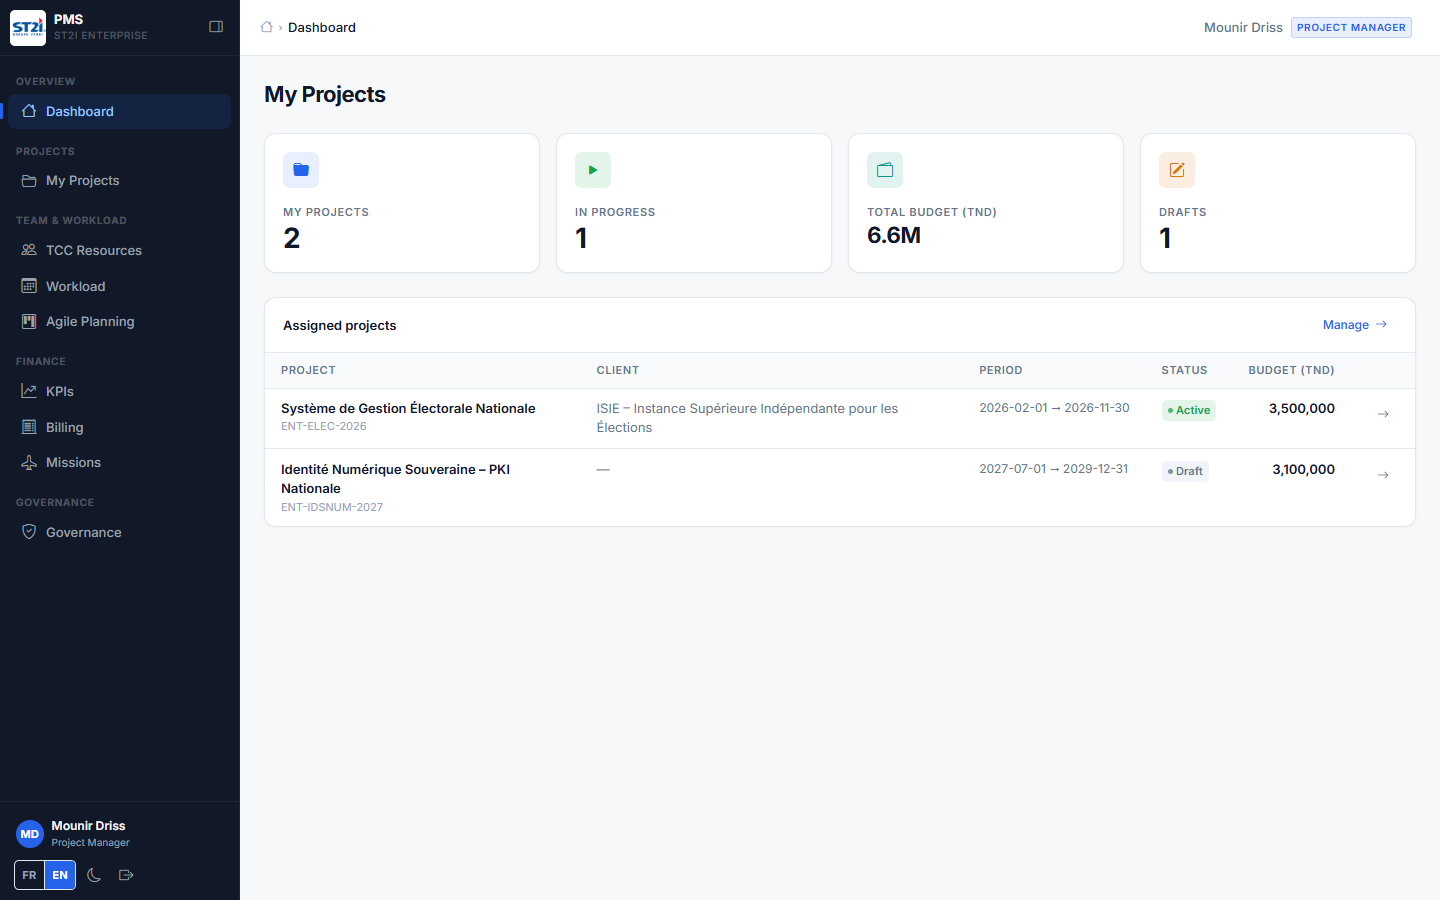
\includegraphics[width=0.92\columnwidth]{img/ui_pm_dashboard.png}
  \caption{Project manager view: the menu carries the finance and governance sections, and the
           workspace is limited to the projects the user manages}
  \label{fig:ui-pm-dashboard}
\end{figure}

\begin{figure}[H]
  \centering
  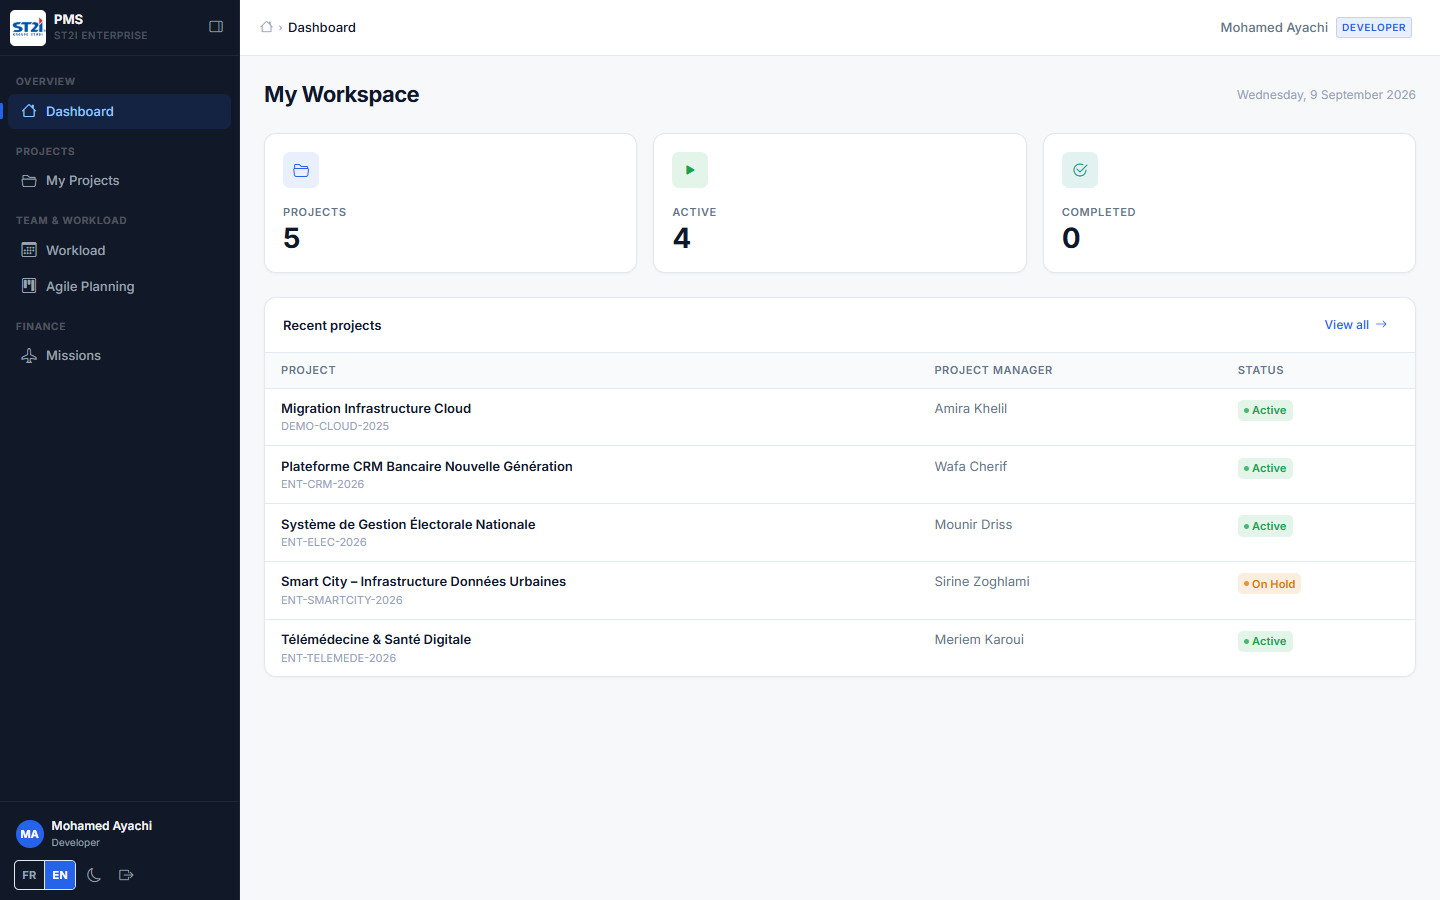
\includegraphics[width=0.92\columnwidth]{img/ui_dev_dashboard.png}
  \caption{Developer view of the same application: no cost rates, no indicators, no billing and no
           governance, because the role holds none of those permission codes}
  \label{fig:ui-dev-dashboard}
\end{figure}

The comparison is the point of the sprint. Nothing distinguishes these two sessions except the
row that links their account to a role, and the rows that link that role to permissions. No branch
in the code names a role, and no menu is hidden by a hard-coded condition: removing
\texttt{VIEW\_KPI} from the developer role removes the entry, and granting it back restores it, in
both cases without recompiling anything. The requirement that a developer must never see the margin
of the project they work on is met by the absence of a row, not by an \texttt{if}.

\subsubsection{Users and resources}
The \texttt{user} module manages accounts, that is creation by the administrator with a temporary
password, modification, activation and deactivation, and role assignment, together with the human
resources and their daily and loaded cost rates. Conversions between entities and data transfer
objects are handled by MapStruct mappers.

\begin{figure}[H]
  \centering
  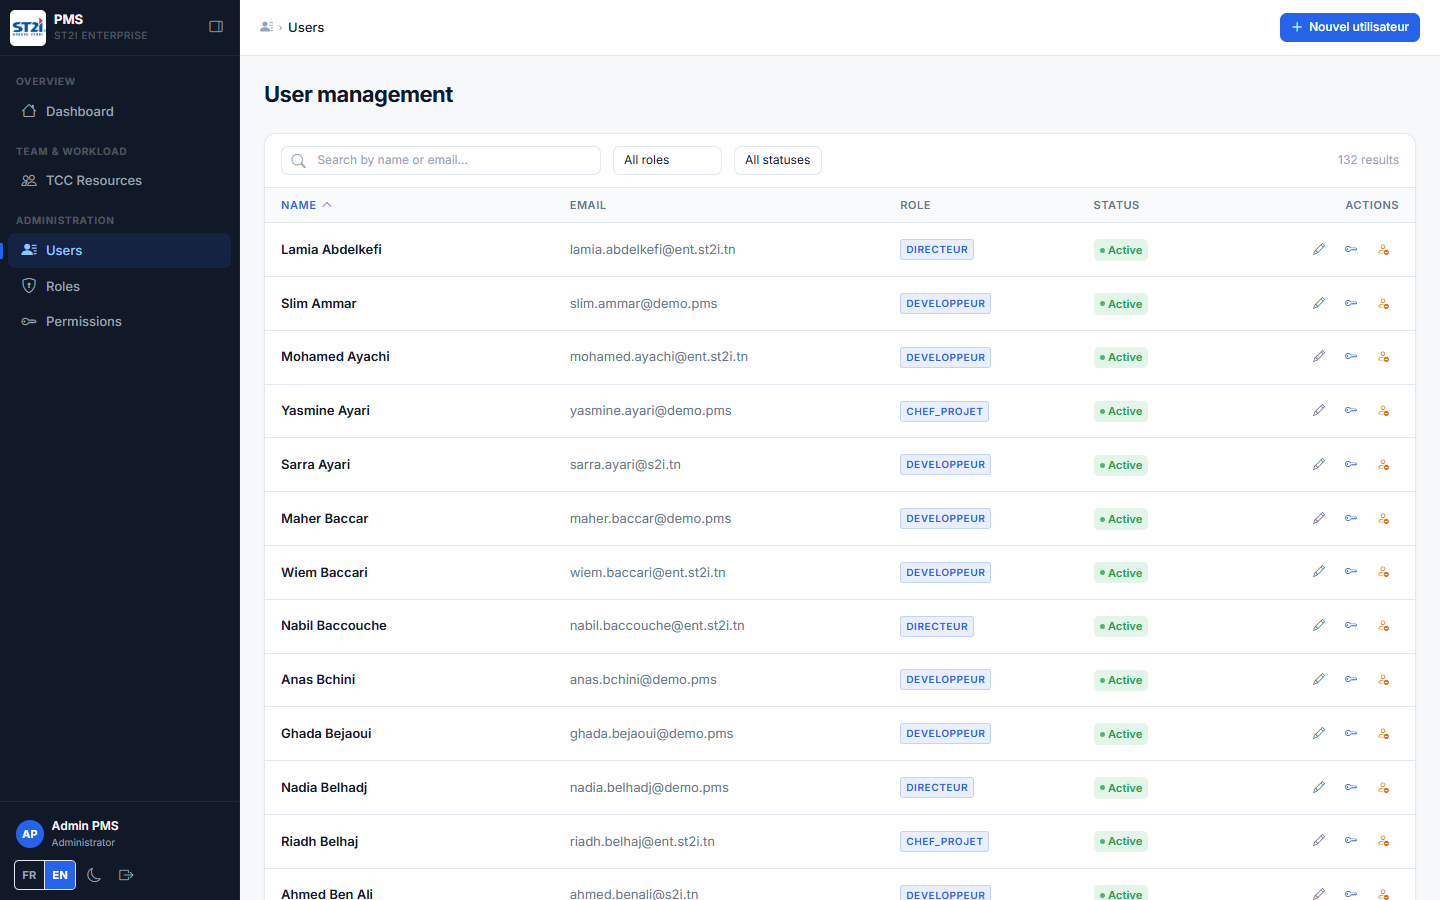
\includegraphics[width=0.9\columnwidth]{img/ui_users.png}
  \caption{User management interface}
  \label{fig:ui-users}
\end{figure}

\begin{figure}[H]
  \centering
  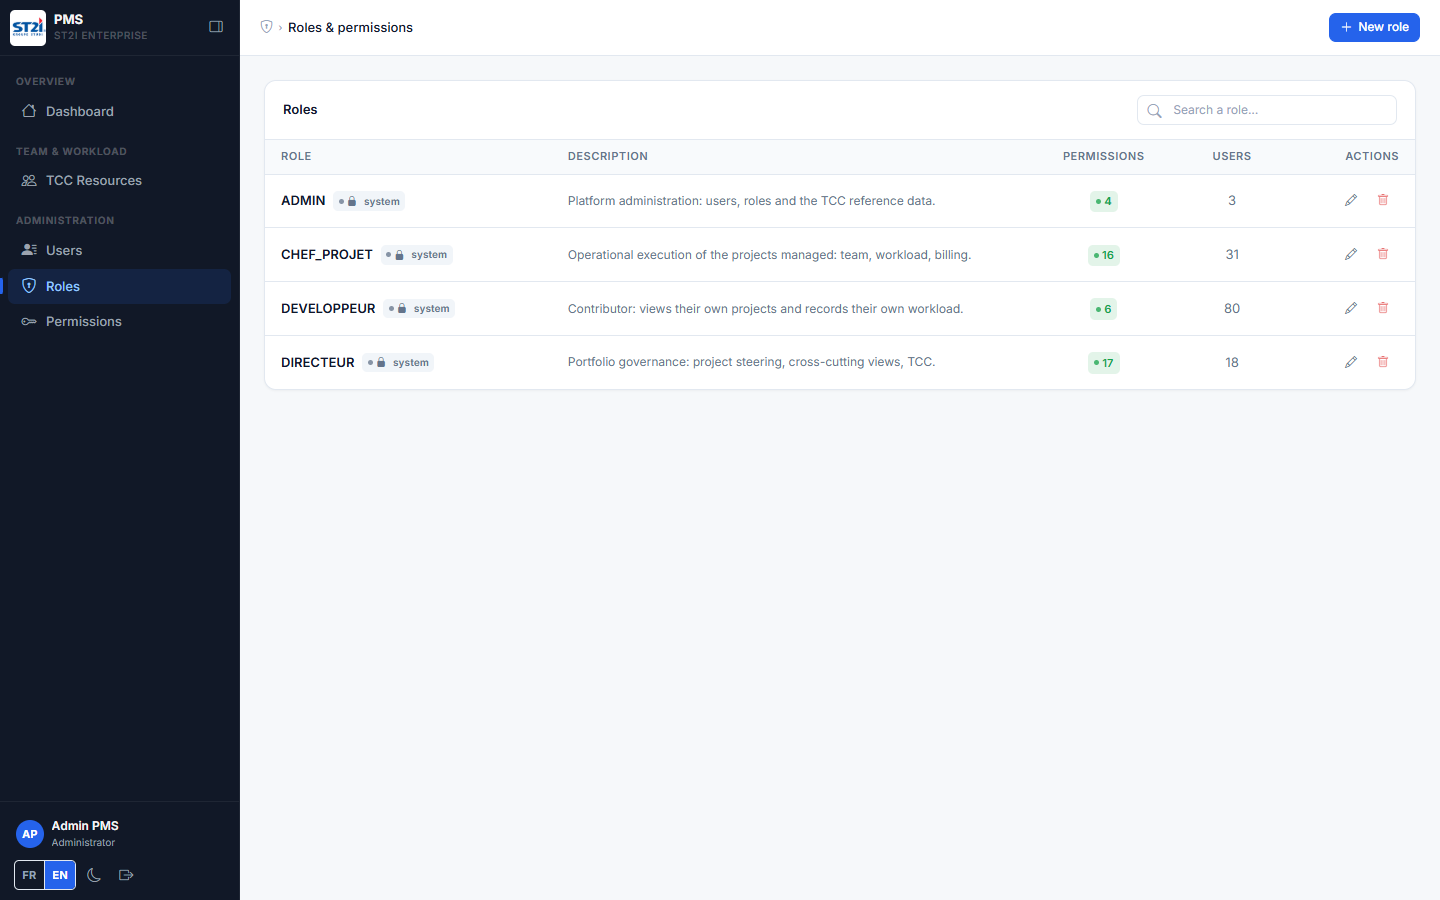
\includegraphics[width=0.9\columnwidth]{img/ui_roles.png}
  \caption{Role and permission management interface}
  \label{fig:ui-roles}
\end{figure}

\begin{figure}[H]
  \centering
  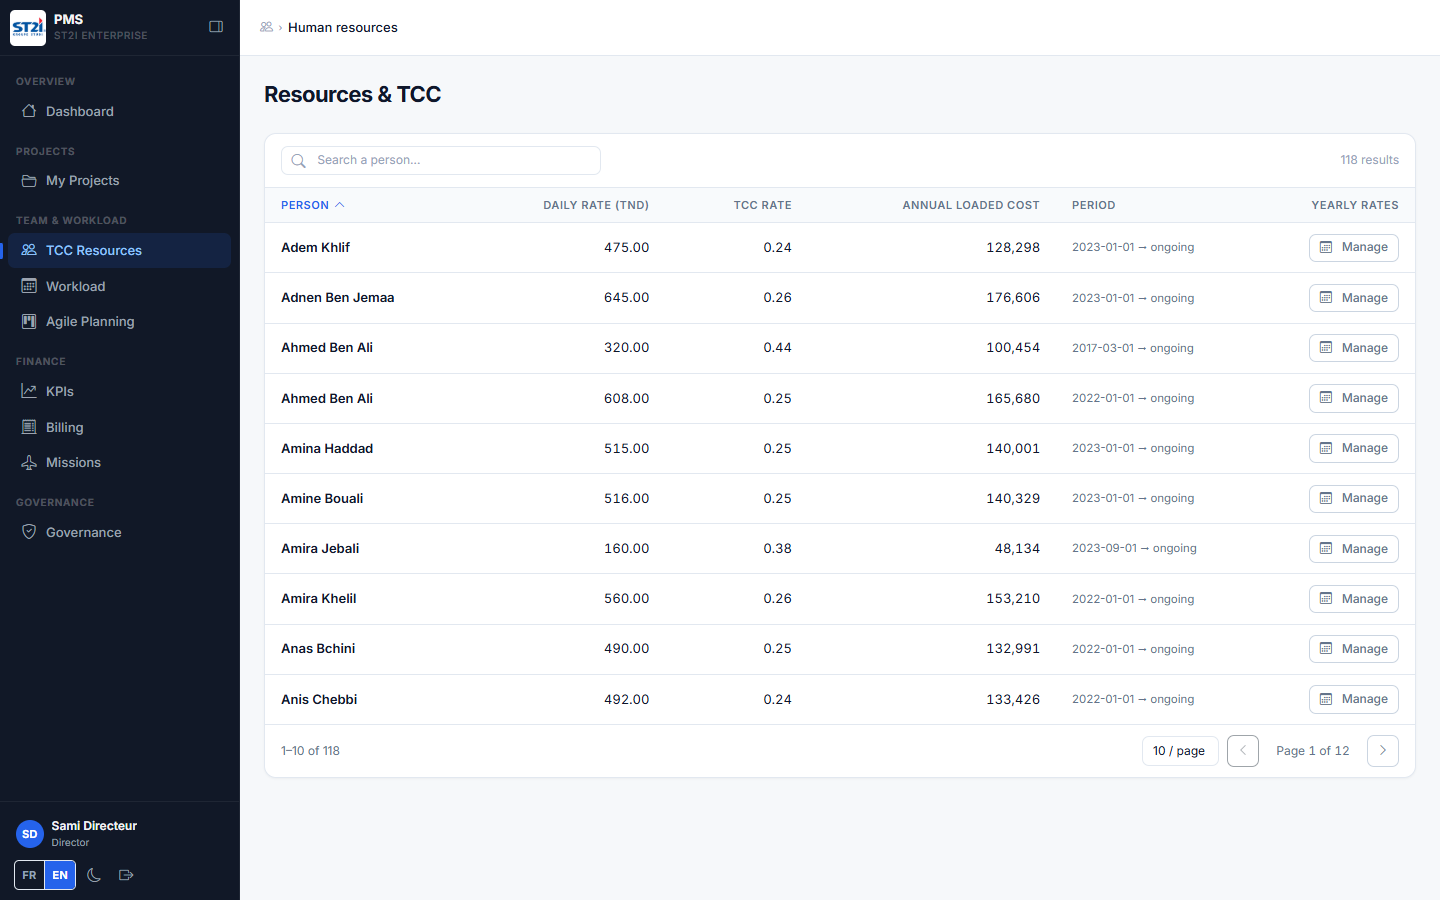
\includegraphics[width=0.9\columnwidth]{img/ui_resources.png}
  \caption{Resource and yearly cost rate interface}
  \label{fig:ui-resources}
\end{figure}

\section*{Conclusion}
Release~1 established the foundations on which the entire platform rests: a modular application
skeleton with auditing and controlled migrations, a robust authentication chain, and above all a
dynamic authorization model that makes the security policy configurable data rather than compiled
code. The platform now knows not only who the user is but what that user may do, and it holds the
reference data the business modules consume. The next release exploits this foundation to deliver
the operational management of projects and workload.
